\documentclass[tikz,border=10pt]{standalone}
\usepackage{pgfplots}
\usepgfplotslibrary{fillbetween}
\pgfplotsset{every axis plot post/.append style =
  {samples=80, smooth, thick, black, mark=none} }
\begin{document}
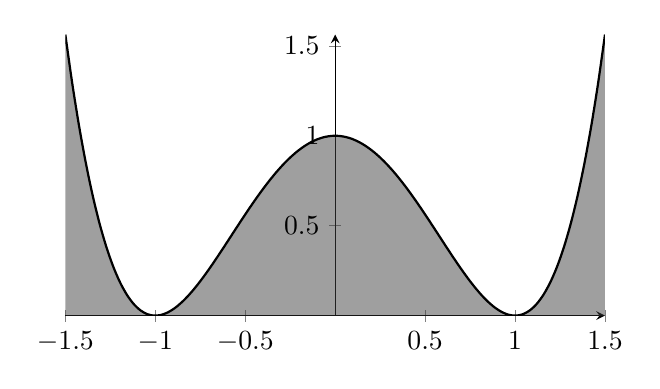
\begin{tikzpicture}
  \begin{axis}[axis lines = center,
    axis equal image, domain = -1.5:1.5]
    \addplot[name path=quartic] {(x^2-1)^2};
    \path[name path=xaxis] (axis cs:-1.6,0)
      -- (axis cs:1.6,0);
    \addplot[darkgray,opacity=0.5]
      fill between[of=quartic and xaxis];
  \end{axis}
\end{tikzpicture}
\end{document}
